\documentclass[a4paper]{article}
% \documentclass[a4paper]{book}

% Imports
\usepackage[utf8]{inputenc}
\usepackage[ngerman]{babel}
\usepackage[T1]{fontenc}
\usepackage{fancyhdr}
\usepackage{caption}
\usepackage{float}
\usepackage{subcaption}
\usepackage{epigraph}
\usepackage{subfiles}
\usepackage[acronym]{glossaries}
\usepackage{graphicx}
\usepackage[style=apa]{biblatex}
\usepackage{pdfpages}
\usepackage{attachfile2}
\usepackage{hyperref}

\bibliography{./Bibliography}

% Generate the glossary
\makeglossaries

% Title page
\title{Open Source Software \\
    \noindent\rule[0.25ex]{\linewidth}{0.5pt}
    \large Wie nehmen Endanwender Open Source Software wahr?
}

\author{
  Blechschmidt, Til\\
  \texttt{til@blechschmidt.de}\\
  Nordakademie, Elmshorn
  \and
  Peeters, Noah\\
  \texttt{noah.peeters@icloud.com}\\
  Nordakademie, Elmshorn
}

% Numbering
\setcounter{secnumdepth}{3}
\setcounter{tocdepth}{2}

% Quote styling
\setlength\epigraphwidth{.8\textwidth}
\setlength\epigraphrule{0pt}

% Glossery
% \newglossaryentry{oss}{name=OSS, description={Open Source Software}}
\newacronym{oss}{OSS}{Open Source Software}


\begin{document}
    % Title page
    \thispagestyle{fancy}
    \maketitle

    % Abstract
    \begin{abstract}
         \gls{oss} wird in vielen Bereichen eingesetzt. In dieser Arbeit wird analysiert, wie Endanwender \gls{oss} wahrnehmen.
    \end{abstract}
    \newpage

    % TOC
    \tableofcontents
    \clearpage

    % --- Content ---
    
                    
    \section{Fragestellung}
        In der Arbeit soll die Frage, inwiefern Endanwender Open Source Software wahrnehmen, untersucht werden. Dabei soll nicht nur die \emph{direkte} Verwendung von Open Source Software, wie es zum Beispiel bei LibreOffice der Fall ist, eine Rolle spielen, sondern auch die \emph{indirekte} Nutzung als Komponente kommerzieller Lösungen wie Chromium bzw. WebKit als Basis von Google Chrome\footcite{is:open:source:right:for:you} aber auch als Werkzeug wie Linux als Betriebssystem für Server\footcite{report:BaselineScenario}.
		
		Es wird erwartet, dass viele Nutzer unbewusst und indirekt mit Open Source Software in Kontakt stehen, sie diese also als Teil größerer, kommerzieller Closed Source Software nutzen, sich dessen aber nicht bewusst sind. Außerdem ist zu erwarten, dass nur ein kleiner Teil der Anwender direkt mit Open Source Software interagiert\footcite{oss:lotus-to-linux}.
		
		Um zuverlässige Daten zu erhalten, die die aktuelle Wahrnehmung der Endanwender widerspiegeln, wird eine Umfrage durchgeführt. Für die Sicherstellung der Repräsentativität der Umfrage werden mindestens 80 Antworten erwartet.
		Die Umfrage wird quantitativ mit geschlossenen Fragen gestaltet, um den Aufwand für die Befragten zu minimieren und damit die Teilnehmerrate und Datenmenge zu maximieren. % TODO: Cite
		
		\subsection{Definitionen} % TODO: Achtung Reihenfolge Definitionen/Fragestellung
            \subsubsection{Open Source Software}
                \begin{quote} 
                    \centering 
                    Software wird als Open Source bezeichnet, wenn ihr Quelltext frei zugänglich ist. Sie kann in kommerzieller Software eingesetzt werden, ihre Nutzung muss allerdings nicht kostenfrei sein. 
                \end{quote}
                
            \subsubsection{Nutzung von Open Source Software}
                Die Nutzung von Open Source Software durch Endanwender kann in zwei Arten unterschieden werden.
                
                \paragraph{Direkte Nutzung}
                    Zum einen gibt es die direkte Nutzung, bei der der Nutzer eine Software verwendet, die Open Source ist, also dessen Source Code frei zugänglich ist.
                    
                    Beispiele für Direkte Nutzung:
                    \begin{itemize}
                        \item Wikipedia\footnote{Wikipedia ist eine Konfiguration von Wikimedia, dessen Source Code frei zugänglich ist (\fullcite{wikimedia:download}).}
                        \item Thunderbird\footnote{\fullcite{thunderbird:faq}}
                        \item ... % TODO: mehr Beispiele
                    \end{itemize}
                    
                \paragraph{Indirekte Nutzung}
                    Zum anderen gibt es die indirekte Nutzung. Hier verwendet der Nutzer Software, dessen Source Code nicht frei zugänglich ist, deren Funktionalität aber entscheidend von \gls{oss} Komponenten abhängt. Ohne diese Komponenten wäre die Funktionalität stark eingeschränkt. Hierbei werden folgende Komponenten \textbf{nicht} berücksichtigt:
                    
                    \begin{itemize}
                        \item Entwicklerwerkzeuge wie Compiler
                        \item Datenbanken wie MySQL
                        \item Betriebssysteme wie Linux 
                        \item ... % TODO: gibt es mehr? Apache Web server?
                    \end{itemize}
                    Der Grund dafür liegt in der Verbreitung dieser Komponenten. % TODO: bessere Erklärung
                    
                    Beispiele für Indirekte Nutzung:
                    \begin{itemize}
                        \item Google Chrome\footnote{\fullcite{chromium:homepage}}
                        \item macOS\footnote{\fullcite{apple:oss}}
                        \item ... % TODO: mehr Beispiele
                    \end{itemize}

            
        
    \section{Design und Durchführung}
		Zweck der Befragung ist es, einen repräsentativen Überblick über die Wahrnehmung von Open Source Software des Endanwenders zu erhalten. Dabei soll Aufschluss über die Verteilung von indirekter sowie direkter Nutzung gegeben werden und in dem Zusammenhang analysiert werden, warum sich Anwender für Open Source Software entscheiden. Außerdem soll evaluiert werden, welche Gründe die Nutzer für und gegen die Nutzung von Open Source Software sehen.
	
		\subsection{Design}
			Die Erhebung ist in vier Teile gegliedert, die im Folgenden näher erläutert sind: 
		   
			\paragraph{Bewusste Nutzung}
				Um die, dem Anwender bewusste, Nutzung von Open Source Software zu erheben, beginnt die Umfrage mit diesem Abschnitt.\\
				Zunächst wird ermittelt, ob die Nutzer wissen, was Open Source Software ist. Um im weiteren Verlauf der Umfrage sinnvolle Antworten zu erhalten, wird anschließend die Definition von Software sowie quelloffener Software erklärt.\\
				Nun werden Fragen zum Nutzungsverhalten von solcher Software gestellt ohne dabei Beispiele zu nennen, um Beeinflussung zu vermeiden.
			
			\paragraph{Unbewusste Nutzung}
				Im zweiten Abschnitt werden konkrete Beispiele für Open Source Software genannt, um die Nutzer darauf aufmerksam zu machen, wo Open Source Komponenten und Softwares überall eingesetzt werden, ohne dass es ihnen klar ist.\\
				Außerdem soll geklärt werden, warum es Differenzen, wenn vorhanden, zwischen bewusster und unbewusster Nutzung gibt.
			
			\paragraph{Gründe für und gegen Open Source Software}
				Im dritten Abschnitt werden Fragen bezüglich der Nutzungs- und Hinderungsgründe von Open Source Software gestellt. Dazu wird gefragt, warum oder warum nicht Endnutzer oder Unternehmen Open Source Software einsetzten. Die möglichen Antworten werden aus der Schweizer Studie zum Thema Open Source\footcite{oss:studie} genommen, um die Wahrnehmung mit der realen Nutzung vergleichbar zu machen.
			
			\paragraph{Demographische Differenzen}
				Zur Analyse von Differenzen innerhalb der Bevölkerungen enthält die Umfrage Fragen zur aktuellen Tätigkeit\footnote{Schüler, Student, Arbeitnehmer, etc.}, dem Geschlecht sowie zur Selbsteinschätzung der Computerkenntnisse.
				
		\subsection{Durchführung}
			Um die Reichweite der Umfrage zu maximieren und die Kosten zu minimieren wird diese in Form einer Onlinebefragung umgesetzt. Dabei werden Kanäle wie Social Media, E-Mail, Messenger genutzt, um auf die Umfrage aufmerksam zu machen. Zudem wird der Link zu der Umfrage über private Kontakte in Schulen und an der Nordakademie verbreitet.
     
    \section{Auswertung}
        \subsection{Vorgehen}
            
    
        \subsection{Wissen über OSS}
            Das Wissen über Open Source Software bei Endanwendern ...
            
            
                
        \subsection{Nutzung von OSS}
            Die Nutzung von OSS bei Endanwendern
        
        \subsection{Gründe für Open Source Software}
            Die Gründe für die Nutzung von Open Source Software aus Sicht der Endanwender
    
    \section{Zusammenfassung}
    
    \clearpage
    \section{Eidesstaatliche Erklärung}
        Hiermit erklären wir, dass wir die vorliegende Hausarbeit selbstständig verfasst und keine anderen als die angegebenen Hilfsmittel benutzt haben.\\
        Die Stellen der Hausarbeit, die andere Quellen im Wortlaut oder dem Sinn nach entnommen wurden, sind durch Angabe der Herkunft kenntlich gemacht. Dies gilt auch für Zeichnungen, Skizzen, bildliche Darstellungen sowie für Quellen aus dem Internet.
        
        
        \begin{figure}[H]
            \centering
            \begin{minipage}{.5\textwidth}
                \centering
                
\includegraphics[width=\textwidth]{assets/signature_tilb.png}
                Til Blechschmidt
                \label{fig:test1}
            \end{minipage}%
            \begin{minipage}{.5\textwidth}
                \centering
                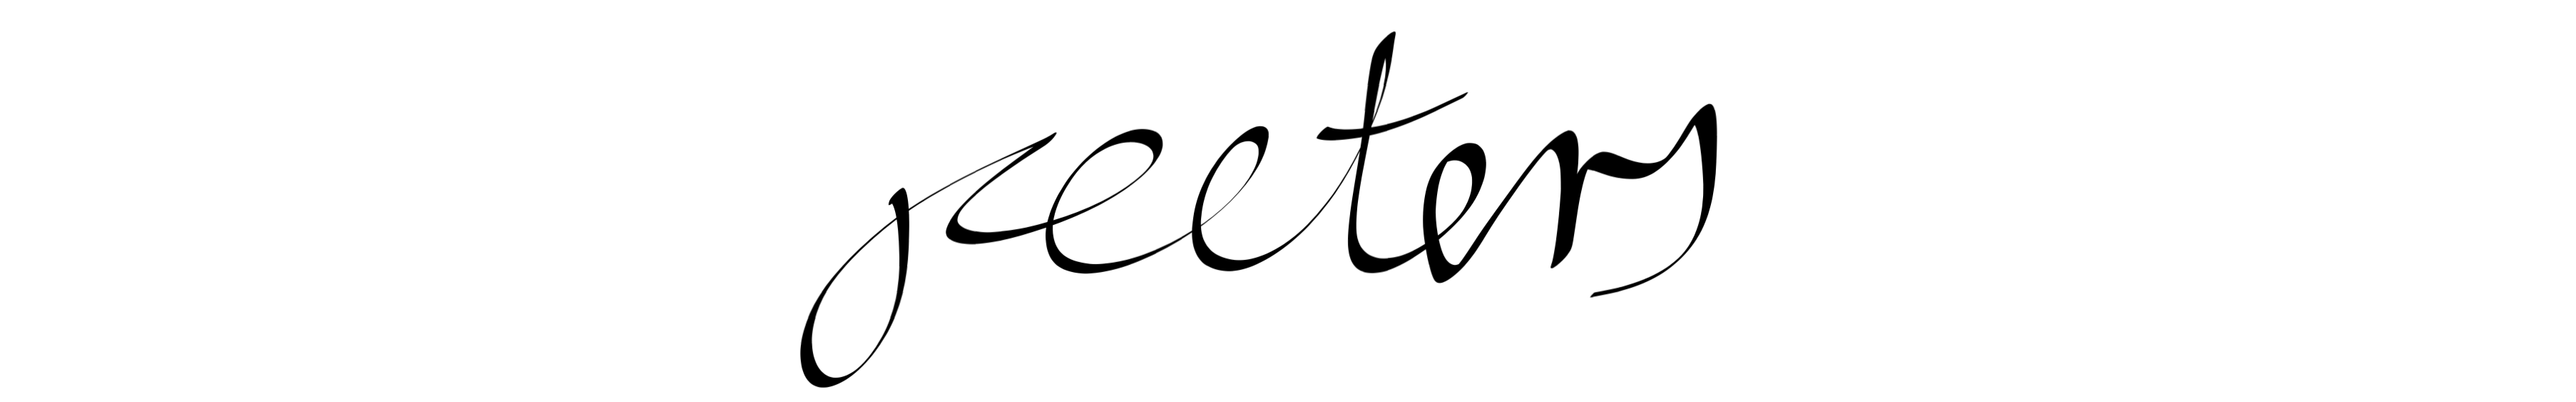
\includegraphics[width=\textwidth]{assets/signature_noahp.png}
                Noah Peeters
                \label{fig:test2}
            \end{minipage}
        \end{figure}
        \clearpage
    
    \clearpage
    \section{Appendix}
        \printglossary[type=\acronymtype]
        \printglossary
        
        \clearpage
        \nocite{*}
        \printbibliography
        
        \clearpage
        
        \subsection{Abschnitte}
            \begin{tabular}{rl}
              Abschnitt & Autor \\
              \hline
              Bla & N. Peeters\\
              Bla & T. Blechschmidt
            \end{tabular}
        
        \subsection{Umfrage}
            \paragraph{Ergebnisse}
                Die Ergebnisse der Umfrage liegen als CSV-Datei bei und sind auch in dieses PDF eingebunden: \attachfile{assets/OpenSource.csv}
            \paragraph{Fragebogen}
                Auf den nächsten vier Seiten befindet sich eine PDF-Version des Fragebogens, wie er Online verbreitet wurde.
                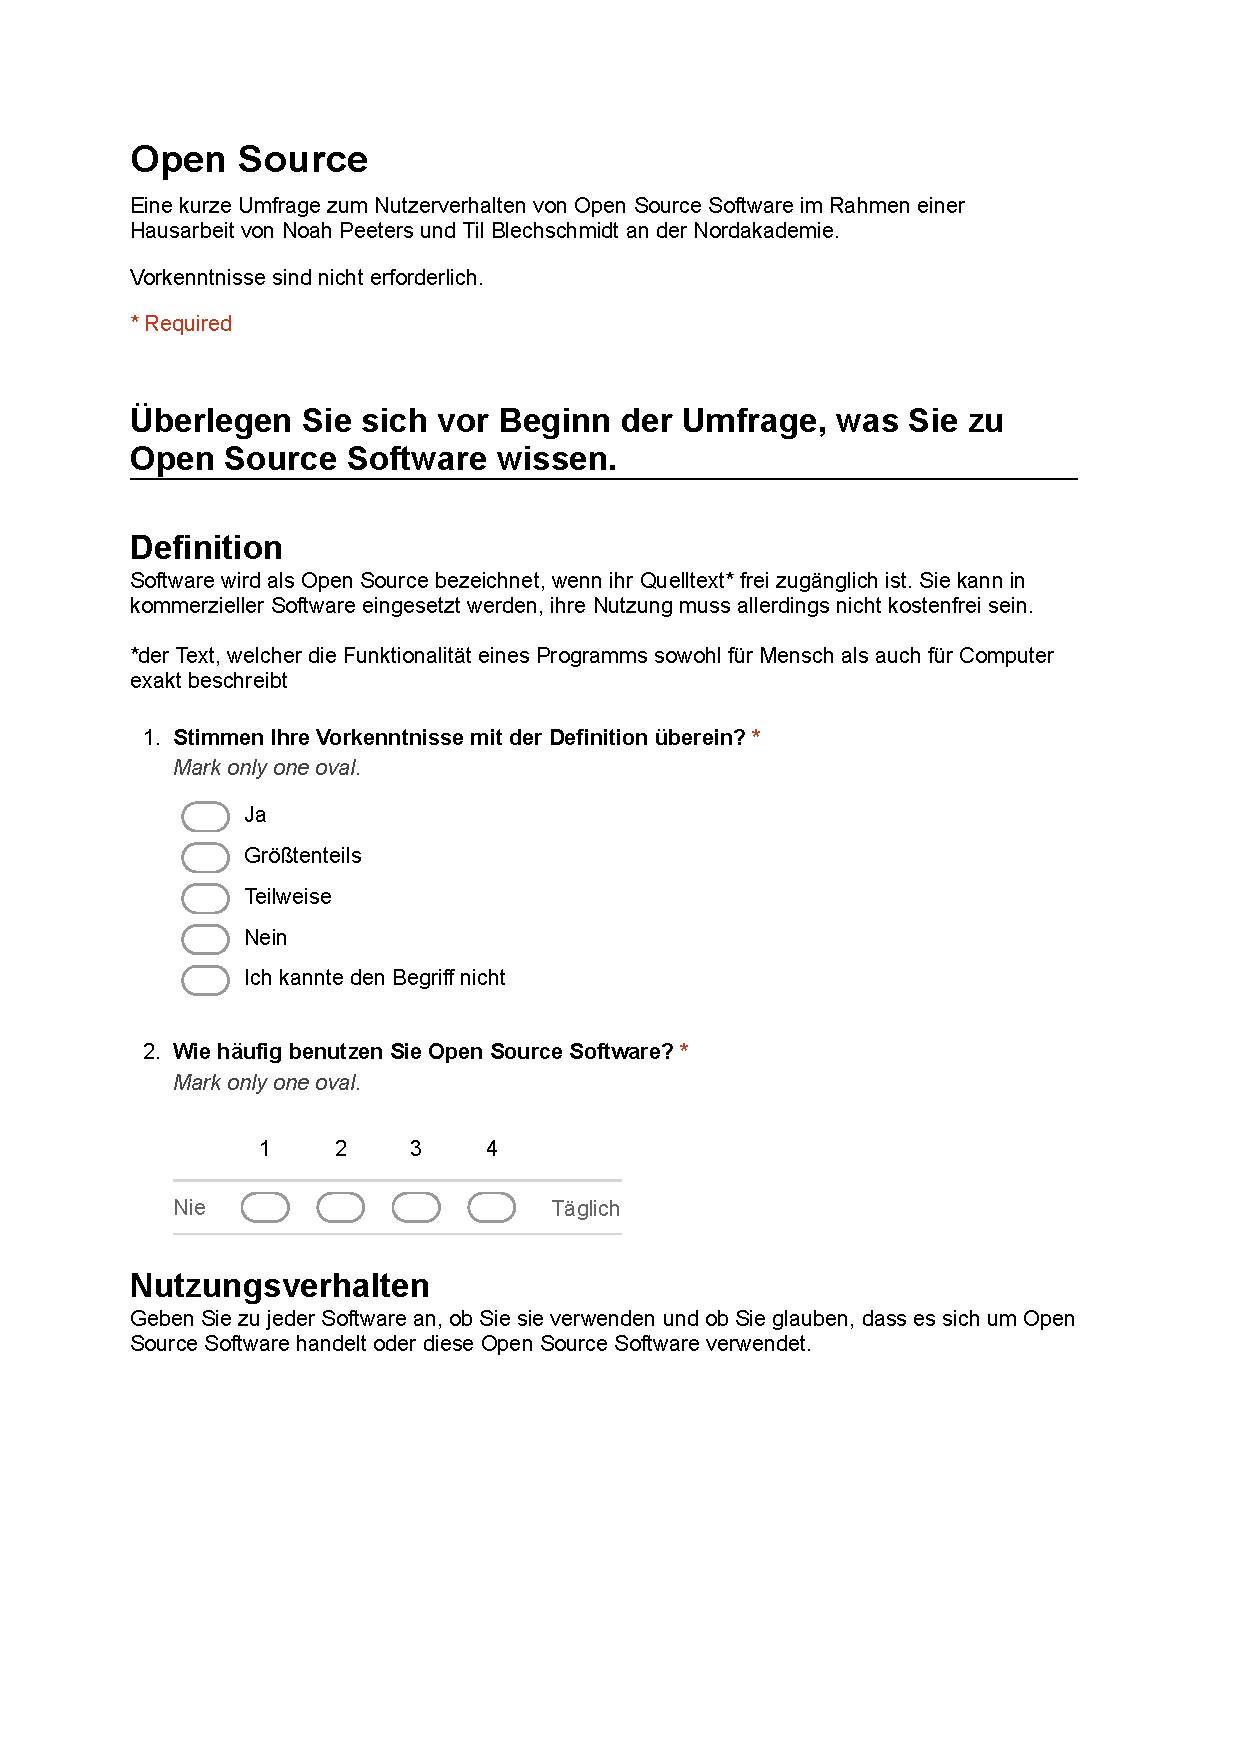
\includepdf[pages={-}]{assets/Umfrage.pdf}

\end{document}
